% Ludwik Ciechański
\documentclass[12pt]{article}
    
\usepackage[T1]{fontenc}
\usepackage{beramono}
\usepackage{polski}
\usepackage[utf8]{inputenc}
\usepackage[a4paper, total={6in, 10in}]{geometry}
\usepackage{listings}
\usepackage[usenames,dvipsnames]{xcolor}
\usepackage{graphicx}
\usepackage{float}
\usepackage{color}
\usepackage{titlesec}
\usepackage[hidelinks]{hyperref}
\usepackage[font=small]{caption}

\newcommand{\cFaculty}[1]{\Large \textsc{#1}\par}
\newcommand{\cSubject}[1]{\Large #1\par}
\newcommand{\cTitle}[1]{\LARGE \textbf{#1}\par}
\newcommand{\cAuthors}[1]{\large #1\par}
\newcommand{\cDate}[1]{\small #1\par}

\setcounter{section}{-1}
\setcounter{figure}{-1}
\graphicspath{ {images/} }
\titlespacing{\section}{0pt}{2pt}{2pt}
\titlespacing{\subsection}{0pt}{3pt}{2pt}

%%
%% Julia definition (c) 2014 Jubobs
%%
\lstdefinelanguage{Julia}
  {morekeywords={abstract,break,case,catch,const,continue,do,else,elseif,
      end,export,false,for,function,immutable,import,importall,if,in,
      macro,module,otherwise,quote,return,switch,true,try,type,typealias,
      using,while},
   sensitive=true,
   alsoother={$},
   morecomment=[l]\#,
   morecomment=[n]{\#=}{=\#},
   morestring=[s]{"}{"},
   morestring=[m]{'}{'},
}[keywords,comments,strings]

\lstset{
  language         = Julia,
  basicstyle       = \fontsize{10}{12}\selectfont\ttfamily,
  keywordstyle     = \bfseries\color{blue},
  stringstyle      = \color{magenta},
  commentstyle     = \color{ForestGreen},
  showstringspaces = false,
  aboveskip=3mm,
  belowskip=3mm,
  numbers=none,
  breaklines=true,
  breakatwhitespace=true,
  tabsize=4,
  frame=shadowbox
}


\begin{document}

% strona tytułowa
\noindent%
\begin{minipage}[t]{.35\textwidth}
    \vspace{0pt}
    
\includegraphics[scale=0.36]{logoAGH}
\end{minipage}%
\begin{minipage}[t]{.65\textwidth}
    \vspace{2pt}
    \cFaculty{Katedra Informatyki}
    \cSubject{Metody obliczeniowe w nauce i technice}
    \vspace{10pt}
    \cTitle{Laboratorium 6 - interpolacja\\ sprawozdanie z ćwiczenia}
    \vspace{10pt}
    \cAuthors{Ludwik Ciechański}
    \cDate{\today}
\end{minipage}
\vspace{30pt}

% --------------------
\section{\bf Przygotowanie}

\subsection{\bf używane pakiety}
\begin{lstlisting}
using Plots
using Polynomials
using DataFrames
using Statistics
using Interpolations
\end{lstlisting}

\subsection{\bf przykładowe dane}
\begin{lstlisting}
# wylosowanie wezlow interpolacji
xs = 1:1:10
A = [rand() for x in xs]
# geste punkty do rysowania wykresow funkcji interpolujacych
xsf = 1:0.02:10
\end{lstlisting}

\subsection{\bf ilustracja}
\begin{center}
    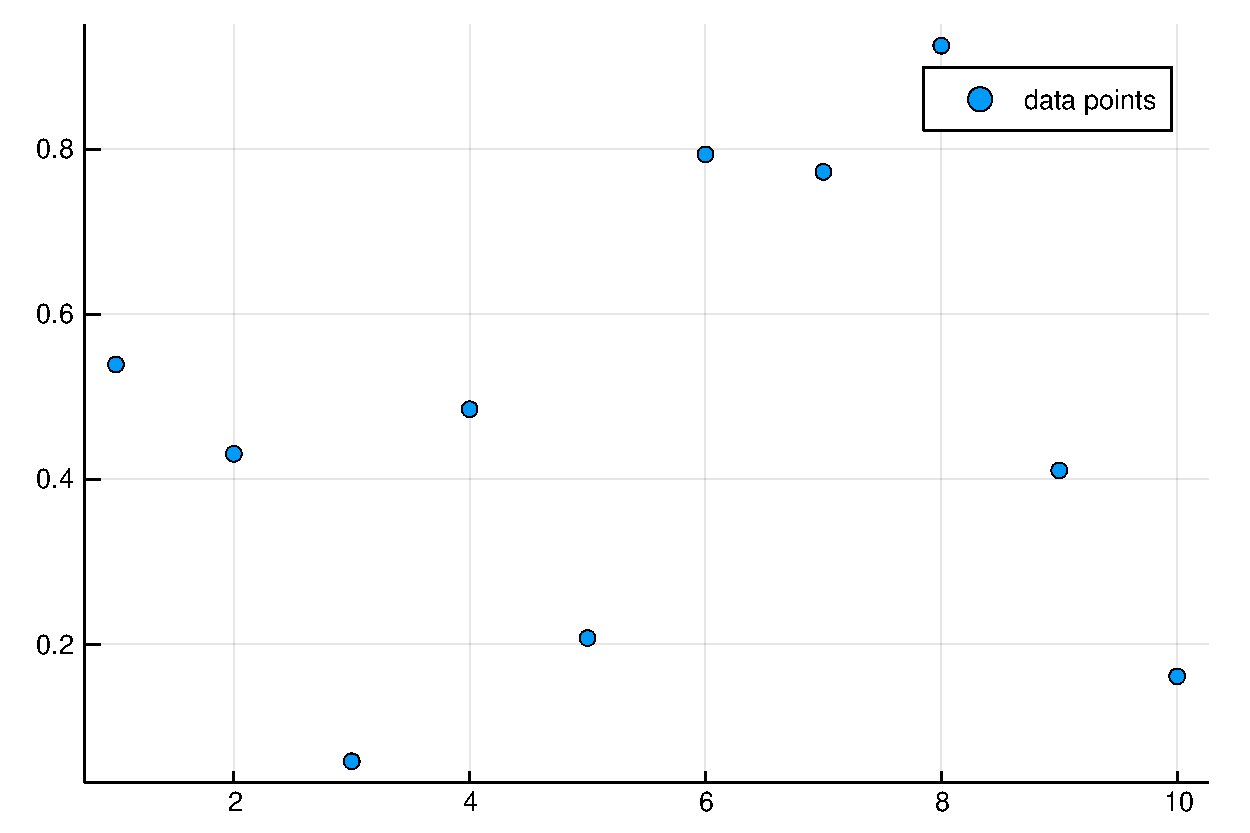
\includegraphics[width=0.89\textwidth]{plot0.pdf}
    \captionof{figure}{Wylosowane węzły interpolacji}
    \label{fig:0}
\end{center}
\clearpage
% ----------------------------------
\section{\bf Wielomian interpolacyjny Lagrange’a}

\subsection{\bf wzory}
$L_k(x) = \displaystyle \prod_{i=0, i \neq k}^{n} \frac{x-x_i}{x_k-x_i}
\qquad P_n(x) = \displaystyle \sum_{k=0}^{n} L_k(x)f(x_k)$

\subsection{\bf kod}
\begin{lstlisting}
function lagrange_interpolation(xs, A)   
    n = size(A,1)
    P = Poly([0])
    for k = 1:n
        l = Poly([1.0])
        for i = 1:n
            if i != k
                l = l * poly([xs[i]]) / (xs[k] - xs[i])
            end
        end            
        P += (l * A[k])
    end
    P
end
\end{lstlisting}
\begin{lstlisting}
fit1 = lagrange_interpolation(xs, A)
B1 = [fit1(x) for x in xsf]
p1 = scatter(xs, A, label="data points")
plot!(xsf, B1, label="lagrange interpolation")
savefig(p1, "img/plot1.pdf")
\end{lstlisting}

\subsection{\bf wykres}
\begin{center}
    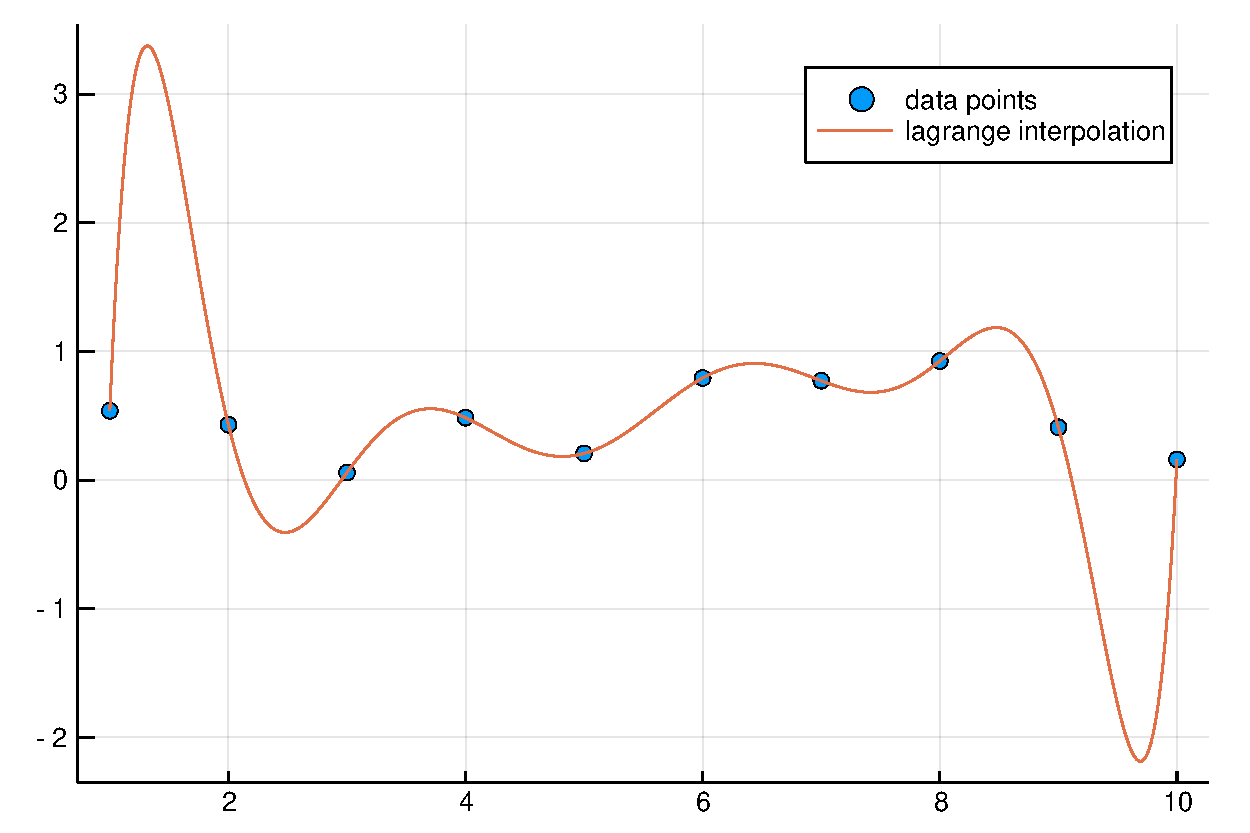
\includegraphics[width=0.99\textwidth]{plot1.pdf}
    \captionof{figure}{Interpolacja wielomianem Lagrange'a}
    \label{fig:1}
\end{center}
\clearpage
% ----------------------------------
\section{\bf Metoda Newtona (ilorazów róznicowych)}

\subsection{\bf wzory}
$w(x) = a_0 + \displaystyle \sum_{i=1}^{n} a_i \prod_{j=0}^{i-1} (x-x_j)$

\subsection{\bf kod}
\begin{lstlisting}
function newton_interpolation(xs, A, n)
    if n == 1
        Poly(float(A[1]))
    else
        prev = newton_interpolation(xs, A, n-1)
        p = A[n] - polyval(prev, xs[n])
        q = 1
        for i = 1:n-1
            q = q * (xs[n] - xs[i])
        end        
        poly([xs[i] for i in 1:n-1]) * (p / q) + prev
    end
end
\end{lstlisting}
\begin{lstlisting}
fit2 = newton_interpolation(xs, A, size(A,1))
B2 = [fit2(x) for x in xsf]
p2 = scatter(xs, A, label="data points")
plot!(xsf, B2, color=:orange, label="newton interpolation")
savefig(p2, "img/plot2.pdf")
\end{lstlisting}

\subsection{\bf wykres}
\begin{center}
    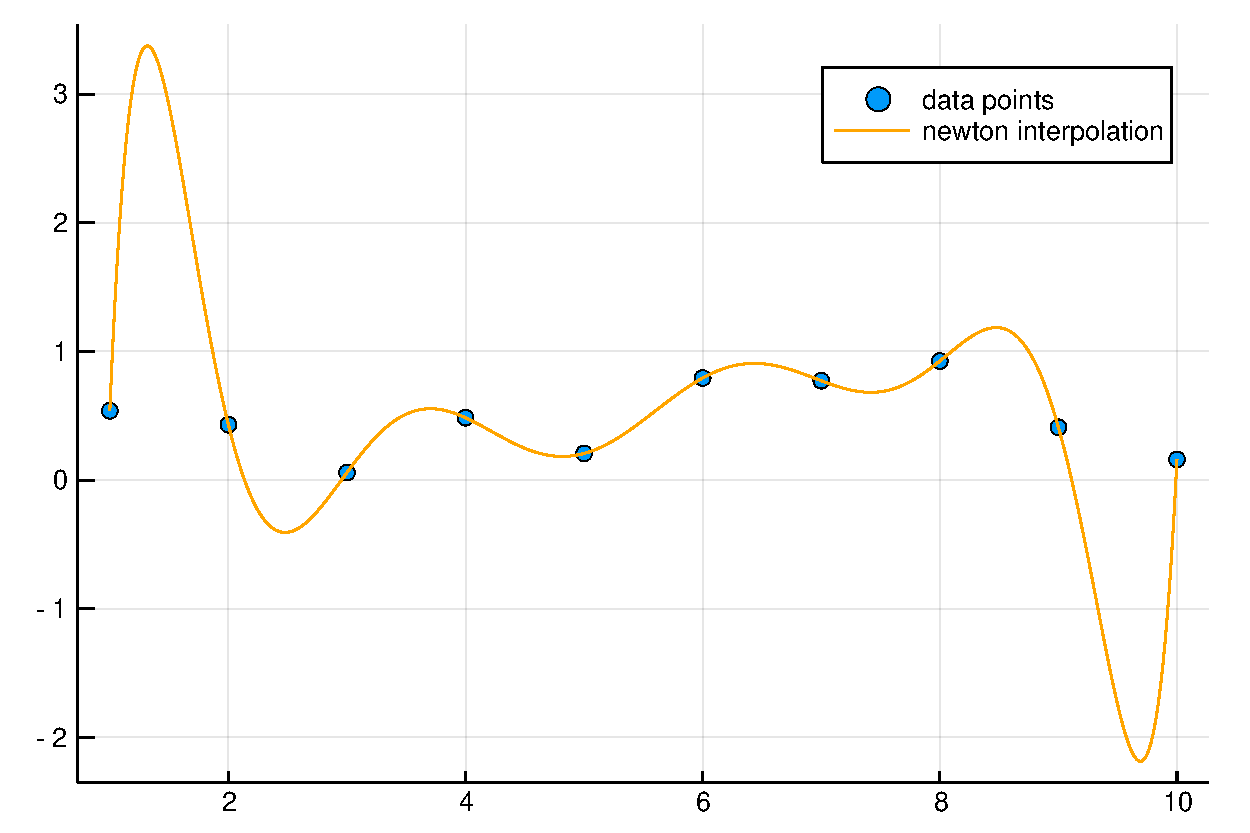
\includegraphics[width=0.99\textwidth]{plot2.pdf}
    \captionof{figure}{Interpolacja metodą Newtona}
    \label{fig:2}
\end{center}
\clearpage
% ----------------------------------
\section{\bf Pakiet Polynomials}

\subsection{\bf wybrane funkcje}
\begin{lstlisting}
Poly(a::Vector) where {T<:Number} 
    # tworzy wielomian na podstawie wspolczynnikow
poly(r::AbstractVector) 
    # tworzy wielomian na podstawie pierwiastkow
polyval(p::Poly, x::Number)
    # oblicza wartosc wielomianu p w punkcie x
polyfit(x, y, n=length(x)-1)
    # dopasowuje wielomian (stopnia n) do punktow (x,y)
    # aproksymacja metoda najmniejszych kwadratow
\end{lstlisting}

\noindent Porównać wszystkie 3 wyniki interpolacji 
wielomianowej na jednym wykresie.
\subsection{\bf kod}
\begin{lstlisting}
fit3 = polyfit(xs, A)
B3 = [fit3(x) for x in xsf]
p3 = scatter(xs, A, label="data points")
plot!(xsf, B1, color=:red, label="lagrange interpolation")
plot!(xsf, B2, color=:orange, label="newton interpolation")
plot!(xsf, B3, color=:green, label="polyfit interpolation")
savefig(p3, "img/plot3.pdf")
\end{lstlisting}

\subsection{\bf wykres}
\begin{center}
    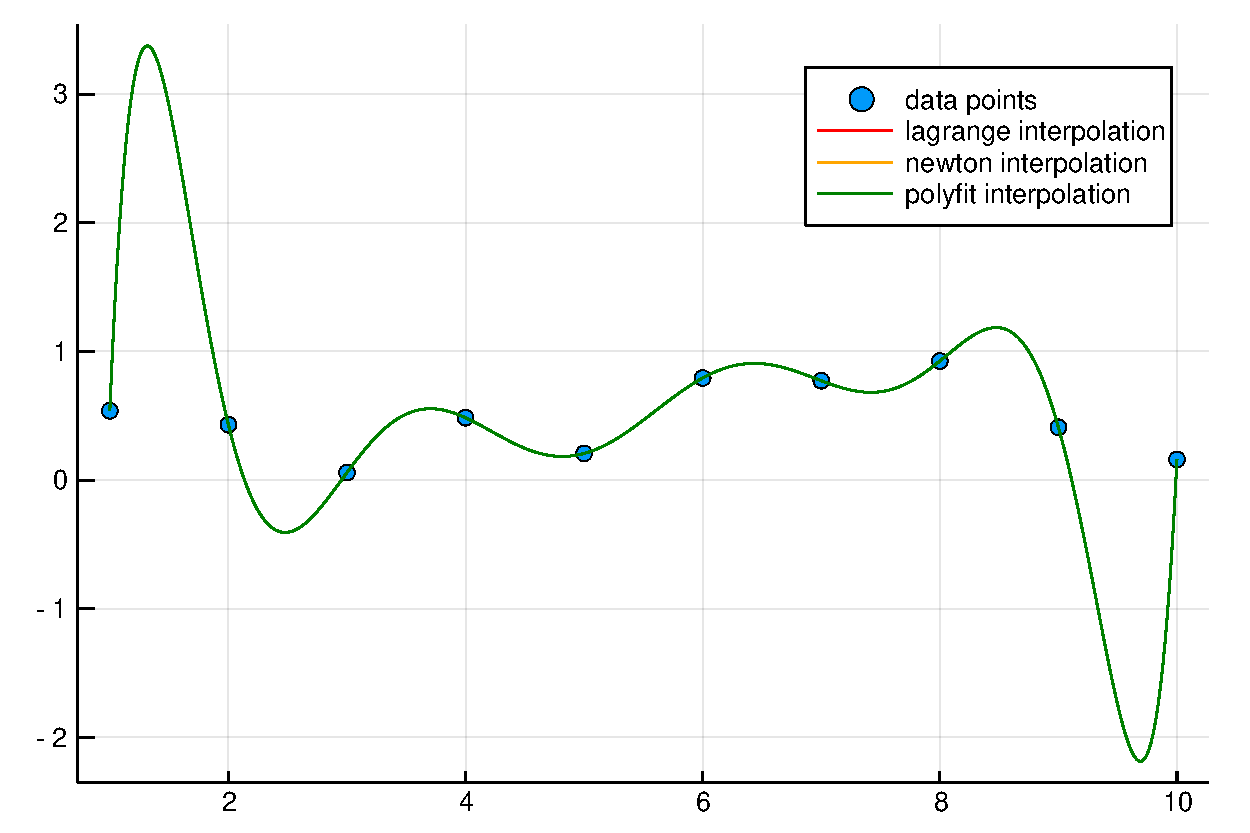
\includegraphics[width=0.97\textwidth]{plot3.pdf}
    \captionof{figure}{Interpolacja polyfit z pakietu Polynomials}
    \label{fig:3}
\end{center}

\noindent Co zauważamy? Niezależnie od zastosowanej metody, dla danych 
węzłów interpolacji wyznaczany jest ten sam wielomian. \\
Dlaczego? Otóż dla $n+1$ punktów istnieje \textit{dokładnie} jeden 
wielomian $n$-tego stopnia interpolujący te punkty.
\clearpage
% ----------------------------------
\section{\bf Porównanie metod}
\noindent Porownać metody poprzez pomiar czasu wykonania dla zmiennej 
ilości węzłow interpolacji. Dokonać pomiaru 10 razy i policzyc wartość 
średnią oraz oszacować błąd pomiaru za pomocą odchylenia standardowego.
\subsection{\bf pomiary}
\begin{lstlisting}
df = DataFrame(size = Int64[], method = String[], time = Float64[])
for r in 100:50:500
    x = 0:1:r
    for i in 1:10
        y = rand(Int, r+1)
        push!(df, [r, "lagrange",@elapsed lagrange_interpolation(x, y)])        
        push!(df, [r, "newton", @elapsed newton_interpolation(x, y, r)])
        push!(df, [r, "polyfit", @elapsed polyfit(x, y)])
    end
end
\end{lstlisting}

\subsection{\bf obliczenia}
\begin{lstlisting}
dfm = by(df, [1,2]) do grouped
    DataFrame(time_mean = mean(grouped[3]), time_std = std(grouped[3]))
end
\end{lstlisting}

\subsection{\bf wykres}
\begin{center}
    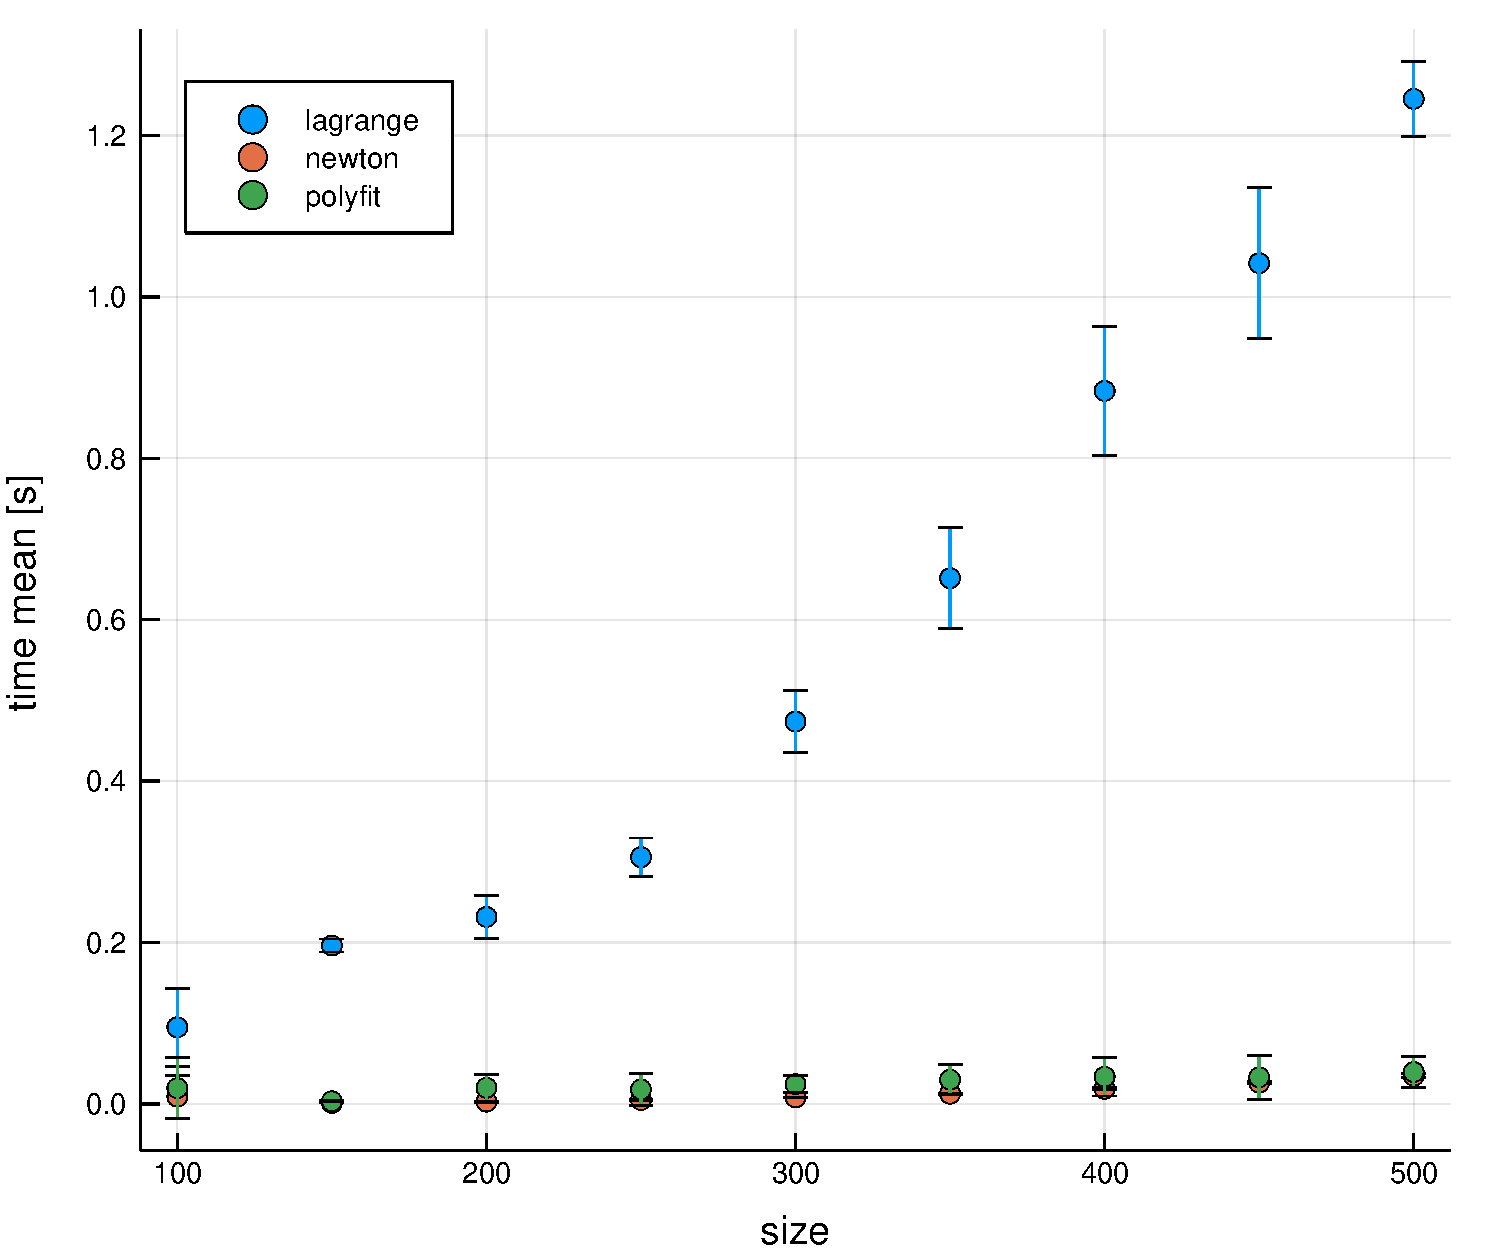
\includegraphics[width=0.99\textwidth]{plot4.pdf}
    \captionof{figure}{Porównanie metod}
    \label{fig:4}
\end{center}
\clearpage
% ----------------------------------
\section{\bf Interpolacja funkcjami sklejanymi}
\subsection{\bf kod}
\begin{lstlisting}
#interpolacja szescienna 
cubic = CubicSplineInterpolation(xs, A)
#interpolacja BSpline'ami
bspline = interpolate(A, BSpline(Linear()))

B5 = [cubic(x) for x in xsf]
B5b = [bspline(x) for x in xsf]
p5 = scatter(xs, A, label="data points", legend=:topright)
plot!(xsf, B5, color=:violet, label="cubic spline interpolation")
plot!(xsf, B5b, color=:orange, label="bspline linear interpolation")
plot!(xsf, B2, color=:grey, label="newton interpolation")
savefig(p5, "img/plot5.pdf")
\end{lstlisting}

\subsection{\bf wykres}
\begin{center}
    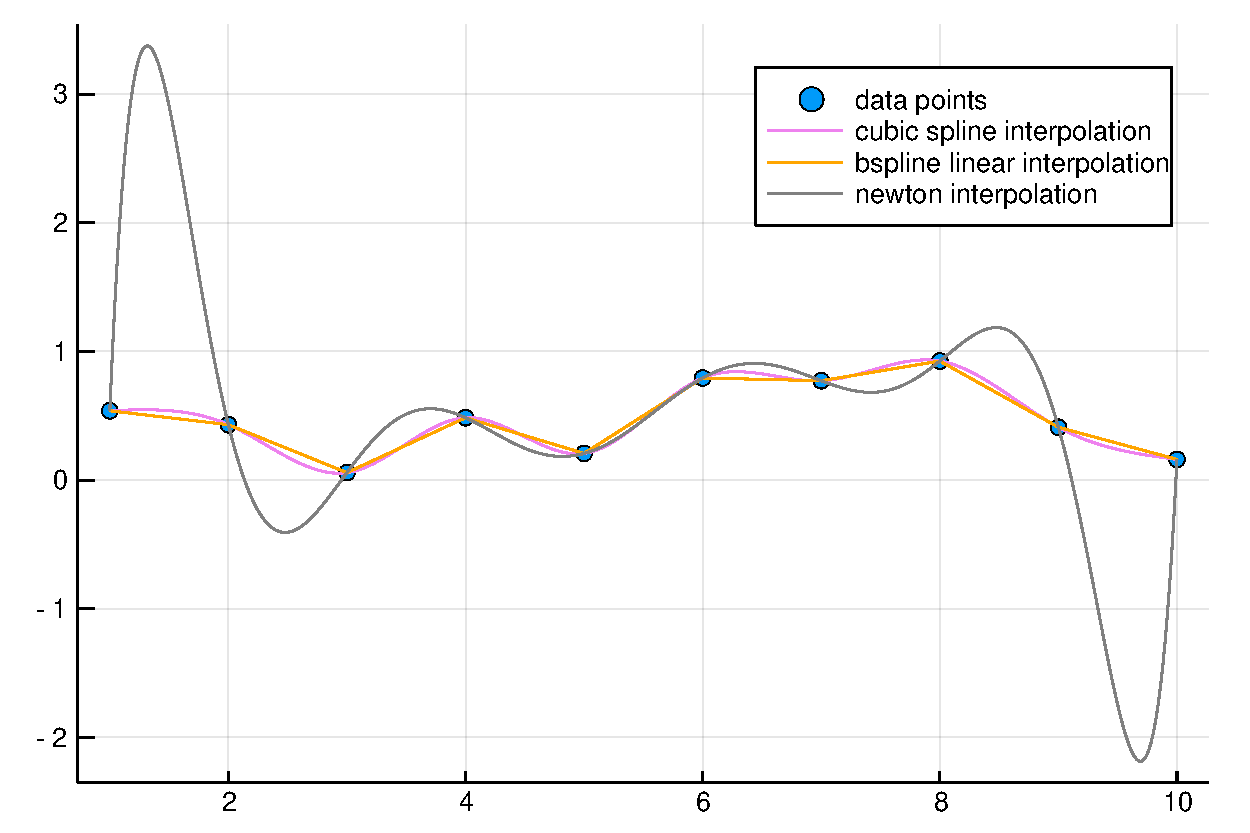
\includegraphics[width=0.99\textwidth]{plot5.pdf}
    \captionof{figure}{Interpolacja funkcjami sklejanymi}
    \label{fig:5}
\end{center}

\section{\bf Efekt Rungego}
\noindent Widoczny jest na rysunku~\ref{fig:5}.\\
Polega na pogorszeniu jakości interpolacji wielomianowej, mimo 
zwiększenia liczby jej węzłów. Początkowo ze wzrostem liczby węzłów 
$n$ przybliżenie poprawia się, jednak po dalszym wzroście $n$, zaczyna 
się pogarszać, co jest szczególnie widoczne na końcach przedziałów.\\
Takie zachowanie się wielomianu interpolującego jest zjawiskiem typowym 
dla interpolacji za pomocą wielomianów wysokich stopni przy stałych 
odległościach węzłów. Występuje ono również, jeśli interpolowana funkcja
jest nieciągła albo odbiega znacząco od funkcji gładkiej. [źródło: wikipedia]
\clearpage
% ----------------------------------
\section{\bf Podsumowanie}
\noindent Jest kilka metod interpolacji wielomianowej. Dla danych węzłów
interpolacji wszystkie zwracają ten sam wielomian 
(rysunki \ref{fig:1}, \ref{fig:2} oraz \ref{fig:3}).
Metoda Lagrange'a jest najwolniejsza spośród badanych.\\
Interpolacja funkcjami sklejanymi daje lepsze efekty niż wielomianowa,
ponadto nie występuje wówczas efekt Rungego.
\vspace{2cm}

% spis tresci
\tableofcontents

\end{document}